%% 
%% Author:  Olivier Fourmaux (olivier.fourmaux@upmc.fr)
%% 


%%%%%%%%%%%%%%%%%%%%%%%%%%%%%%%%%%%%%%%%%%%%%%%%%%%%%%%%%%%
%% Type et package

\documentclass[a4paper,12pt]{article}

\usepackage[francais,english]{babel}
\usepackage{fancyhdr}
\usepackage[latin1]{inputenc}
\usepackage{epsfig}
\usepackage{calc}
\usepackage{url}
\usepackage{boxedminipage}

%%%%%
%%Rajout
\usepackage{epstopdf}
\usepackage{enumerate}
\usepackage{cite}
%\usepackage{hyperref}
\renewcommand{\FrenchLabelItem}{\textbullet}
\usepackage[babel=true]{csquotes}
\usepackage[T1]{fontenc}


\newenvironment{changemargin}[2]{%
\begin{list}{}{%
\setlength{\leftmargin}{#1}%
\setlength{\rightmargin}{#2}%
}%
\item[]}
{\end{list}}

\newcommand{\fig}[1]{Fig.~\ref{#1}}


%%%%%%%%%%%%%%%%%%%%%%%%%%%%%%%%%%%%%%%%%%%%%%%%%%%%%%%%%%%
%%%%%%%%%%%%%%%%%%%%%%%%%%%%%%%%%%%%%%%%%%%%%%%%%%%%%%%%%%%
%% D�finitions � personnaliser 

%% Pour les noms, utilisez la premi�re lettre du pr�nom suivi du 
%% nom de famille (premi�re lettre majuscule, reste en minuscule).


%%%% Indiquer le nom de l'encadrant ci-dessous:

\def\nomEncad{S.~Secci,\\ Y.~Bencha�b, M.~Coudron}
%%<matthieu.coudron@lip6.fr>,
%%<yacine.benchaib@lip6.fr>
%% Si le projet est co-encadr� indiquer les deux noms � la suite dans 
%% Le m�me champs


%%%% Indiquer les noms des �tudiants participant ci-dessous:

\def\nomEtudC{Q.~Dubois}
\def\nomEtudB{K.~Lam}
\def\nomEtudA{R.~Ly}
\def\nomEtudD{S.~Ravier}

%% Si le projet est encadr� par moins de 4 �tudiants laissez
%% les variables inutiles vides


%%%% Indiquer la r�f�rence (numero) et le nom du sujet ci-dessous:

\def\refProjet{9} \def\titreProjetCourt{perf\,MPTCP\,OpenFlow}
\def\titreProjetLong{MPTCP\\Performances et optimisation de la
  s�curit� avec un ordonnancement r�parti dans les topologies
  virtualis�es OpenFlow}

%% Le titre court ne doit pas faire plus d'une vingtaine de caract�re
%% r�sumez le � quelques mots essenciels


%%%% Indiquer le type de document et sa version ci-dessous:

\def\typeDoc{Rapport interm�diaire}
 
%% - Rapport interm�daire
%% - Rapport final



%%%%%%%%%%%%%%%%%%%%%%%%%%%%%%%%%%%%%%%%%%%%%%%%%%%%%%%%%%%
%%%%%%%%%%%%%%%%%%%%%%%%%%%%%%%%%%%%%%%%%%%%%%%%%%%%%%%%%%%
%% D�finitions � ne pas modifier
 
%%%%% ||| Mise en page verticale ||| 
\setlength{\voffset}{-1in} % a4:reste 297mm pour les 5 suivants:
\setlength{\topmargin}{15mm}         % avant l'en-t�te
\setlength{\headheight}{20mm}        % hauteur de l'en-t�te 
\setlength{\headsep}{10mm}            % entre l'en-t�te et le corps
\setlength{\textheight}{220mm}       % hauteur du corps
\setlength{\footskip}{12mm}          % pied de page par rapport au corps 

%%%%% --- Mise en page horizontale ---
\setlength{\hoffset}{-1in} % a4:reste 210mm 
\setlength{\oddsidemargin}{25mm}     % entre hoffset et le corps
\setlength{\evensidemargin}{25mm}    % entre hoffset et le corps
\setlength{\marginparwidth}{0mm}     % largeur de la marge
\setlength{\marginparsep}{0mm}       % s�parateur corps marge
\setlength{\textwidth}{160mm}        % largeur du corps

\def\annee{2013-14}



%%%%%%%%%%%%%%%%%%%%%%%%%%%%%%%%%%%%%%%%%%%%%%%%%%%%%%%%%%%
%% D�but du document

\begin{document}

\selectlanguage{francais}



%%%%%%%%%%%%%%%%%%%%%%%%%%%%%%%%%%%%%%%%%%%%%%%%%%%%%%%%%%%
%% D�finition des en-t�tes et pied de pages
\pagestyle{fancyplain}
\lhead[\fancyplain{}{\texttt{Universit� Pierre et Marie Curie}\\
          Master Informatique\\ UE \textbf{PRes} f�v. \annee \\ \nomEncad}]
      {\fancyplain{}{\textsc{Universit� Pierre et Marie Curie}\\
          Master Informatique\\ UE \textbf{PRes} \annee \\ \nomEncad}}
\chead[\fancyplain{}{\textbf{Projet \refProjet\\\titreProjetCourt}}]
      {\fancyplain{}{\textbf{Projet \refProjet\\\titreProjetCourt}}}
\rhead[\fancyplain{}{\nomEtudA\\\nomEtudB\\\nomEtudC\\\nomEtudD}]
      {\fancyplain{}{\nomEtudA\\\nomEtudB\\\nomEtudC\\\nomEtudD}}
\lfoot[\fancyplain{}{\epsfig{figure=UPMC_sorbonne.eps,width=3cm}}]
      {\fancyplain{}{\epsfig{figure=UPMC_sorbonne.eps,width=3cm}}}
\cfoot[\fancyplain{}{\textbf{\thepage/\pageref{fin}}}]
      {\fancyplain{}{\textbf{\thepage/\pageref{fin}}}}
\rfoot[\fancyplain{}{\typeDoc}]
      {\fancyplain{}{\typeDoc}}

%%%%%%%%%%%%%%%%%%%%%%%%%%%%%%%%%%%%%%%%%%%%%%%%%%%%%%%%%%%

~

      \begin{center}
        \begin{boxedminipage}{12cm}{
            \begin{center}
              ~\\\LARGE\textbf{\titreProjetLong}\\
              ~\\\large Encadrants: \textbf{\nomEncad,}\\
              ~\\\large Etudiants: \textbf{\nomEtudA, \nomEtudB, \nomEtudC, \nomEtudD}\\
              ~
            \end{center}
            }
        \end{boxedminipage}
      \end{center}

~

\tableofcontents
\section{Cahier des charges}

\subsection{Objectifs}
\label{sec:charges:intro}

Les objectifs du projet sont de :
\begin{itemize}
\item mesurer les performances de MPTCP sur diff�rentes topologies de
  r�seaux virtuels.
\item modifier l'ordonnanceur de MPTCP pour privil�gier une
  r�partition �quilibr�e sur les diff�rents sous-flots.
\end{itemize}

\subsection{Contexte}
\label{sec:charges:contexte}

MPTCP est une extension de TCP qui permet pour une connexion TCP
donn�e d'utiliser plusieurs chemins pour l'�change de donn�es. La
multiplicit� des sous-flots a pour but d'am�liorer le d�bit et
d'augmenter la r�silience de la connexion\cite{rfc6182,rfc6824,
  coudroncross2013}.

Les performances de MPTCP ne doivent pas �tre inf�rieures � celles de
TCP et son l'utilisation ne doit pas diminuer le d�bit des autres
utilisateurs s ur le m�me r�seau. Les performances de MPTCP d�pendent
en partie de l'algorithme utilis� pour la r�partition des donn�es
entre les diff�rents sous-flots ouverts \cite{pareto2013}. Pour
caract�riser les performances de l'ordonnanceur de MPTCP, nous allons
le tester dans diff�rents r�seaux virtualis�s en utilisant dans un
premier temps l'algorithme impl�ment� dans le kernel MPTCP de
linux\footnote{\url{mptcp.org}}.

L'emploi de MPTCP am�liorerait la s�curit� si les donn�es transitaient
de mani�re �quilibr�e entre les diff�rents sous-flots, ce qui
complexifient les attaques. Le d�bit global de la connexion serait
affect� car les chemins les plus lents vont ralentir le d�bit des
chemins les plus rapides, ce qui, en contre partie, peut s'av�rer
moins performant qu'une simple connexion TCP.  Nous allons modifier
l'ordonnanceur afin de garantir la r�partition �quitable des charges
puis analyser l'influence de cette modification sur les performances
de MPTCP dans les topologies r�seaux utilis�es pr�c�demment.

\subsection{M�thodes}
\label{sec:charges:methodes}

La r�alisation du projet peut �tre subdivis� en trois parties :
\begin{itemize}
\item la simulation de r�seaux � topologies diff�rentes,
\item l'analyse des performances de MPTCP,
\item l'adaptation de l'ordonnanceur pour l'aspect s�curit�.
\end{itemize}

Nous utiliserons Mininet afin de simuler les topologies r�seaux o�
nous pourrons mesurer les performances de MPTCP � l'aide de l'API
Python fournie par Mininet.  Pour caract�riser l'influence de
l'ordonnanceur sur les performances, nous utiliserons des r�seaux
simples o� les diff�rents sous-flots sont asym�triques et diff�rent
par une propri�t� � la fois : latence, d�bit, pertes... Nous testerons
diff�rents algorithmes de r�partition de charge entre sous-flots :
l'algorithme impl�ment� par d�faut (LIA), celui qui satisfait
l'optimum de pareto par rapport aux objectifs de MPTCP, ou encore un
algorithme de r�partition �quilibr�e de la charge r�seau entre les
diff�rents sous-flots.



\section{Plan de d\'eveloppement}
\label{sec:plan:devt}

La premi�re partie est de consuitre les topologies de diff�rents
r�seaux virtuels et de tester les performances de MTPCP en faisant
varier les param�tres des sous-flots. La seconde partie est de
construire un algorithme d'ordonnancement r�pondant � un crit�re de
s�curit� simple: rendre le \emph{sniffing} des paquets plus
difficile � r�aliser.

\vspace{0.5cm}

Les �tapes du d�veloppement suivront les points suivants:

\begin{itemize}
\item Pr�paration d'une machine mininet avec le noyau MPTCP compil�
  pour l'ensemble de l'�quipe;
\item Lecture, compr�hension et commentaires du code de MPTCP;
\item Pr�paration de plusieurs topologies : une topologie simple �
  plusieurs n\oe uds et un \emph{fat tree} pour simuler un \emph{data
    center};
\item Pr�paration d'une biblioth�que de tests et de mesures via l'API python;
\item \'Ecriture d'un algorithme d'ordonnancement dans le noyau;
\item Mesures de performance.
\end{itemize}

\vspace{1cm}

Le d�veloppement sera divis� en trois sous-projets:

\paragraph{Scripts de tests mininet} Le but de ce sous-projet est
d'�tablir une base pour tester les performances de MPTCP en fonction
des param�tres du r�seau virtuel. Cette base sera r�utilis�e pour les
topologies plus complexe (sous-projet \emph{fat-tree}) ou pour la
mesure de performances du nouvel algorithme
d'ordonnancement. (sous-projet algorithme d'ordonnancement).

\vspace{1cm}
\textbf{Responsable du sous-projet}: M. Ly.

\begin{itemize}
\item Cr�ation d'une machine virtuelle contenant le noyau MPTCP;
\item �criture des scripts pour les simulations et l'analyse;
\item tests sur une topologie simple.
\end{itemize}

\paragraph{\emph{fat tree}}
Ce sous-projet vise � mesurer les performances sur une topologie
complexe o� MPTCP a une utilit� substantielle.


\vspace{1cm}
\textbf{Responsable du sous-projet}: M. Ravier.

\begin{itemize}
\item Cr�ation d'une topologie \emph{fat tree};
\item tests.
\end{itemize}

\paragraph{\'Ecriture d'un algorithme d'ordonnancement}
Ce sous-projet vise � comprendre le code de MPTCP et � �crire un
nouvel algorithme d'ordonnancement, puis � le compiler dans le noyau
Linux.


\vspace{1cm}
\textbf{Responsables du sous-projet}: M. Lam et M. Dubois.

\begin{itemize}
\item Lecture et compr�hension du code;
\item �criture d'un nouvel algorithme d'ordonnancement;
\item d�bogage.
\end{itemize}





\subsection{Scripts de tests mininet}
\begin{figure}[!htb]
  \begin{changemargin}{-2.0cm}{0.5cm}
    \centering
    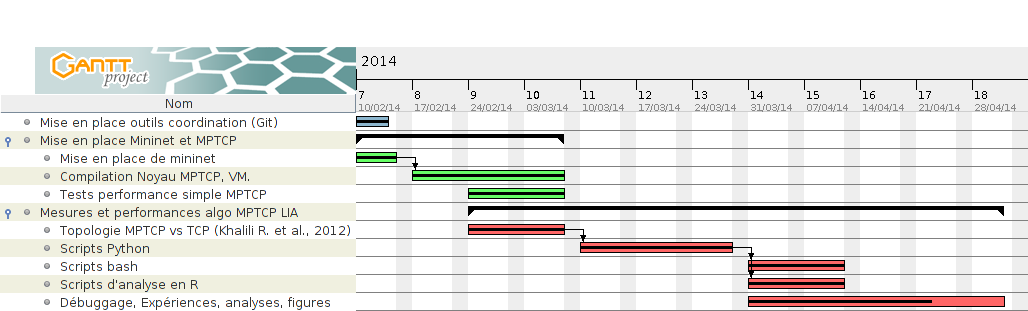
\includegraphics[width=1.2\textwidth]{../gantt/romain.png}
  \end{changemargin}
  \centering
  
  \caption{\textbf{Diagramme de Gantt de Romain Ly.}}
  \label{fig:gantt}
  
\end{figure}

\begin{itemize}
\item Mise en place du Git
\item Compilation noyau MPTCP dans la VM mininet et tests simples de routines
\item Topologie modifi�e de Khalili et al.
\item Scripts Python
  \begin{itemize}
  \item impl�mentation d'un parseur d'arguments
  \item int�gration de ping, iperf, iperf3, bwm-ng, sshd, tcpdump
    permettant le monitoring et l'�tude du r�seau
  \end{itemize}
\item Installation de TCP-reduce dans la VM pour v�rifier les options de la connexion TCP.
\item Scripts Bash pour g�n�rer de multiples simulations par l'interm�diaire de scripts Python
\item Scripts R pour analyse des r�sultats et figures
\item D�bogages des scripts
\item Exp�rimentations
  \begin{itemize}
  \item variation du nombre de sous flots, d�bits, latences, taille de
    fen�tre, etc.
  \end{itemize}
\end{itemize}


\subsection{Topologie \emph{fat-tree}}

\begin{figure}[!htb]
  \begin{changemargin}{-2.0cm}{0.5cm}
    \centering
    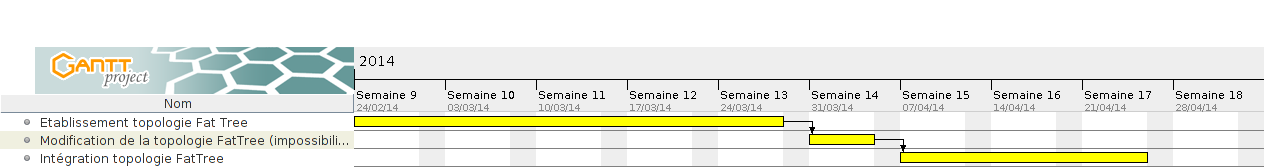
\includegraphics[width=1.2\textwidth]{../gantt/Simon.png}
  \end{changemargin}
  \centering
  
  \caption{\textbf{Diagramme de Gantt de Simon Ravier.}}
  \label{fig:gantt}
\end{figure}

\vspace{1cm}
\begin{tabular}{lp{12cm}}
  03/03 au 30/03 & �tablissement de la topologie FatTree\\
  31/03 au 06/04 & modification de la topologie FatTree (impossibilit� technique de r�aliser le premier mod�le)\\
  07/04 au 27/04 & Int�gration de la topologie FatTree dans
l'environnement de tests (configuration des h�tes, �tablissement des
tables de routage) et r�alisation des tests
\end{tabular}
\vspace{0.5cm}

\subsection{\'Ecriture d'un nouvel algorithme d'ordonnancement}
\begin{figure}[!htb]
  \begin{changemargin}{-2.0cm}{0.5cm}
    \centering
    \includegraphics[width=1.2\textwidth]{../gantt/KevinQuentin.png}
  \end{changemargin}
  \centering
  
  \caption{\textbf{Diagramme de Gantt Kevin Lam et Quentin Dubois}. }
  \label{fig:gantt}
\end{figure}

Analyse de la structure de l'impl�mentation :
	\begin{itemize}
		\item D�terminer globalement les fichiers � lire ;
		\item D�finir les headers et structures li�s � l'utilisation de mptcp.
	\end{itemize}\\

Lecture et Compr�hension du code :
	\begin{itemize}
   		\item Lecture de tous les fichiers contenus dans \$(SRC\_NOYAU)/net/mptcp ;
   		\item Lecture de certains fichiers contenus dans \$(SRC\_NOYAU)/net/sched ;
	   \item Lecture de tous les types/structures utilis�s ;
	   \item Relecture du code apr�s avoir compris tous le types/structures.
	\end{itemize}\\

D�finition des parties modifiables de l'ordonnanceur :
	\begin{itemize}
	   \item V�rifier les correspondances entre mptcp\_output.c et mptcp\_input.c ;
	   \item Voir si l'utilisation du contr�le de congestion (mptcp\_olia.c et mptcp\_coupled.c) a des effets de bord sur les sockets ;
	   \item Voir les diff�rences entre les diff�rents modes du path\_manager.
	\end{itemize}\\

Impl�mentation / Tests d'algorithmes pour l'ordonnanceur :
	\begin{itemize}
		\item Avec l'aide de Matthieu Coudron, modification dans
		\$(SRC\_NOYAU)/net/mptcp/mptcp\_output.c ;
	   \item Tests des impl�mentations avec le travail de Romain LY et comparer les r�sultats obtenus.
   	\end{itemize}\\


\clearpage
\section{Contexte technologique}
\label{sec:contexte-techno}
%// -*- coding: iso-8859-1 -*-

L'�laboration de MPTCP a �t� motiv�e par l'observation de l'existence
dans les r�seaux de plusieurs chemins entre deux machines A et
B. L'utilisation de ces diff�rents chemins entre les deux h�tes
pourrait �tre un atout non n�gligeable pour augmenter le d�bit de la
connexion et/ou la r�silience de la connexion si l'un des chemins
venaient � ne plus pouvoir acheminer les paquets (congestion, panne de
routeur, etc). De plus le multi-chemin permet d'�quilibrer la
r�partition des charges sur les sous-flots utilis�s. TCP n'a pas �t�
con�u pour exploiter plusieurs chemins d'o� la n�cessit� de concevoir
des protocoles multi-chemins comme MPTCP permettant d'utiliser les
chemins disponibles pour transmettre les paquets d'une connexion entre
A et B via les sous-flots connect�s.

Il existe d�j� plusieurs protocoles proposant d'utiliser plusieurs
chemins. Nous en citerons que deux: SCTP et ECMP. SCTP (\emph{Stream
  Control Transmission Protocol}) allie l'avantage de TCP et UDP
(utilisation de datagrammes) et permet de multiplexer les flux sur
plusieurs interfaces \cite{rfcsctp}. ECMP (\emph{Equal Cost
  MultiPath}) est un sous-protocole dans le cadre de divers protocoles
de routages (comme OSPF, TRILL, ...) et qui est utilis� dans les
\emph{data-centers}: lors d'une connexion entre deux h�tes, le routeur
peut transf�rer les paquets sur plusieurs meilleurs chemins � co�ts
\og �gaux \fg{} \cite{rfcecmp}. \\
Les inconv�nients de SCTP est la n�cessit� que tous les h�tes
terminaux puissent comprendre le protocole ; il est donc n�cessaire de
modifier la couche application pour pouvoir l'utiliser. De plus, les
\emph{middle boxes} (pare-feu, NAT, \ldots) ne reconnaissent pas le
protocole et rejettent donc tous les paquets SCTP. ECMP utilise les
routeurs pour conna�tre les chemins et l'augmentation de performance
li� � son utilisation n'est pas significative.

L'avantage principal de MPTCP est d'�tre r�trocompatible par rapport �
TCP.  Si un h�te n'est pas compatible avec MPTCP, la connexion
utilisera TCP r�solvant les probl�mes des \emph{middle boxes}. Le
scond avantage est qu'il est totalement transparent pour les routeurs,
c'est une connexion \emph{end to end}.


\subsection{Fonctionnement de MPTCP}
\label{subsec:fonctMPTC}

MPTCP utilise dans un premier temps une connexion TCP pour cr�er des
sous-flots similaires � TCP avec des chemins diff�rents. La couche TCP
est alors remplac�e par la couche MPTCP qui est divis�e en deux
parties (\fig{fig:mptcpstack}): la couche sup�rieure correspond aux
fonctions n�cessaires � MPTCP de fonctionner (d�couverte et gestion
des chemins, ordonnancement des paquets, contr�le de congestion) et la
couche inf�rieure correspond aux sous-flots �tablis.

\begin{figure}[!htb]
    \centering
    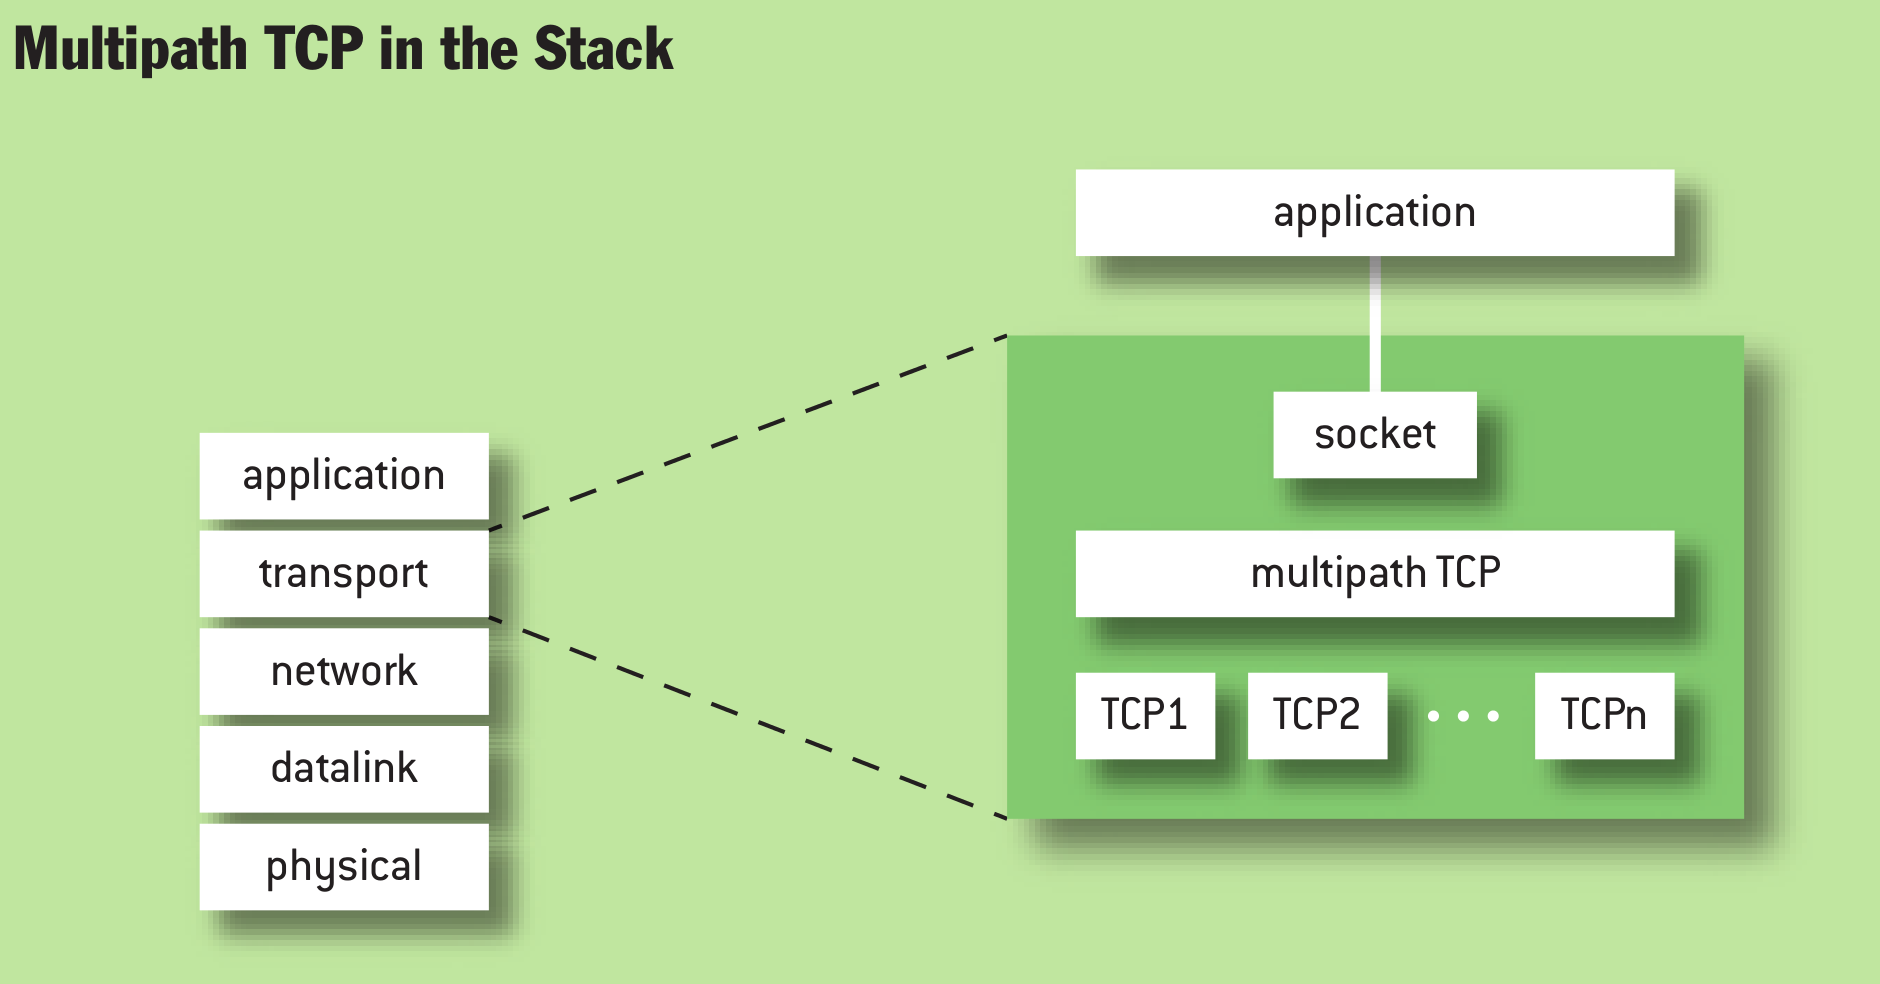
\includegraphics[width=0.8\textwidth]{../figures/mptcp_stack/mptcp_stack.png}
    \caption{\textbf{Sch�ma de la pile MPTCP} \cite{PB14}.}
  \label{fig:mptcpstack}
  
\end{figure}

MPTCP permet l'augmentation du d�bit de mani�re � ce qu'il soit
sup�rieur � une connexion TCP unique sur le meilleur des chemins
disponibles. Il permet aussi la r�silience de la connexion en cas de
panne ou de congestion, dans ce cas le trafic est alors r�parti et/ou
r�exp�di� sur les autres sous-flots sans la n�cessit� de r�tablir une
connexion TCP entre les deux terminaux. Cette approche permet de
r�partir les charges sur les ressources disponibles.

MPTCP impl�mente plusieurs fonctions pour contr�ler les sous-flots de
la connexion \cite{rfc6182}:
\begin{itemize}
\item le gestionnaire de chemin ou \emph{path manager} 
\item l'ordonnanceur de paquets ou \emph{packet scheduling} puis
\item le contr�leur de congestion  ou \emph{congestion controller}.
\end{itemize}

Le sous-flot prend en charge les segments de l'ordonnanceur pour
l'envoyer sur un chemin disponible. Le sous-flot agit comme une
connexion TCP classique et dispose de cette mani�re des fonctions de
ce protocole de transport assurant d'envoyer des paquets de mani�re
fiable et s�quenc�e. \`A la r�ception, le sous-flot envoie les
segments � la couche ordonnanceur de paquet pour le
r�assemblage. Mais, le r�assemblage est d'autant plus rapide si les
paquets re�us sont d�j� bien ordonn�s. Dans ce cas, avoir un
ordonnanceur, qui permet d'estimer le temps d'arriv�e des paquets
selon un sous-flot pour que le r�cepteur re�oive tous les paquets des
diff�rents sous-flots de fa�on ordonn�e permettrait d'augmenter les
performances de MPTCP. En effet, les donn�es dans le buffer seraient
trait�s plus efficacement. Cela affecte donc sur la quantit� de
donn�es pouvant \^etre envoy�es et/ou sur le nombre de sous-flots
exploitables.

Le gestionnaire des chemins est le m�canisme permettant de d�tecter et
d'utiliser les chemins disponibles par l'interm�diaire de multiples
adresses IPs dans les h�tes. Il signale l'existence d'adresses
alternatives et permet d'int�grer de nouveaux sous-flots � une
connexion MPTCP existante ou d'en enlever.

L'ordonnanceur des paquets d�coupe le flux de donn�es provenant de la
couche application en segments pr�ts � �tre envoy�s par l'un des
sous-flots. Il s�quence les segments et permet de r�associer les
segments pour r�ordonner les donn�es c�t� destinataire. L'ordonnanceur
d�pend des informations des chemins disponibles provenant du
gestionnaire de chemins \cite{rfc6356}.

Enfin, le contr�le de congestion est un outil essentiel qui permet
d'adapter le d�bit de chaque sous-flot et de d�finir si un chemin est
trop lent par rapport au meilleur sous-flot. Il permet aussi de
renvoyer l'information au gestionnaire s'il y a une panne.

\vspace{0,5cm}

Le contr�le de congestion n�cessite un algorithme performant pour que
l'utilisation de MPTCP � la place de TCP puisse effectivement
augmenter le d�bit de l'utilisateur sans influencer le d�bit des
autres utilisateurs sur les m�mes chemins, c'est � dire qu'il doit
garantir l'optimalit� de pareto (c'est � dire que l'allocation des
ressources est r�alis�e de mani�re ce qu'il soit impossible
d'augmenter le d�bit d'un utilisateur sans diminuer le d�bit d'un
tiers ou sans augmenter le co�t de la congestion. Il garantit aussi la
r�partition �quitable de la capacit� du lien entre les utilisateurs
\cite{pareto2013}).  L'algorithme de MPTCP est donc un point central
dans les performances de MPTCP sur le r�seau.

Lors des choix des sous-flots, l'algorithme doit effectuer un
compromis entre �quilibre des charges dans les diff�rents sous-flots
et r�activit� (\emph{responsiveness}) en cas de modification de la
latence des sous-flots ou de d�couverte de nouveaux chemins. Une
priorit� vers l'�quilibre des charges entra�ne l'envoi des donn�es sur
les meilleurs routes (selon la m�trique utilis�e, par d�faut la
latence du chemin) mais cela peut d�clencher un changement constant de
route produisant un effet de battement (\emph{flappiness}): si
plusieurs chemins poss�dent le m�me co�t, l'algorithme aura tendance �
changer plus souvent de chemins. Si la priorit� utilis�e est la
r�activit� (par augmentation de la taille de la fen�tre d'un des
sous-flot), l'utilisation de toutes les ressources disponibles peut ne
pas �tre optimale car on aura tendance � utiliser qu'un seul
sous-flot. Les param�tres de l'algorithme doivent �tre d�termin�s
efficacement pour r�partir les charges sur les sous-flots et ne pas
�tre agressif (augmentation trop rapide de la taille de la fen�tre sur
un des sous-flots) pour garantir l'optimalit� de Pareto
\cite{pareto2013}.

 Dans l'algorithme par d�faut, le crit�re privil�gi� par l'algorithme
est le RTT. Il serait int�ressant de modifier les caract�ristiques du
r�seau pour mesurer les performances de MPTCP sur le choix des chemins
utilis�s ou en cas de modification de chemins sur des crit�res de
latence, pertes, d�bit \ldots



\subsection{Utilisation r�elle de MPTCP}
\label{subsec:utilisation}

Dans la pratique, l'utilisation de MPTCP est difficile. L'utilisation
de plusieurs sous-flots ne garantie pas l'augmentation de d�bit. Pour
cel�, il est n�cessaire que les sous-flots empruntent des chemins
physiques diff�rents et aujourd'hui il n'est pas possible pour un
utilisateur de contr�ler le routage de ses paquets de bout en
bout. Une m�thode pour contourner le probl�me serait d'utiliser la
conjonction de MPTCP et de LISP (\emph{Locator/Identifier Separation
  Protocol}) qui permet de d�couvrir la diversit� de chemins existant
entre routeurs de bordures (A-MPTCP)
\cite{coudroncross2013}. 

Cependant il existe des cas o� MPTCP est utilisable � son plein
potentiel et suscite l'int�r�t : dans les datacenters et en
environnement mobile. Par l'interm�diaire d'une strat�gie de routage
par SDN (\emph{Software Defined Network}) par exemple OpenFlow, le
contr�leur peut �tablir des chemins diff�rents entre deux h�tes sur
tout son r�seau. Le transfert de donn�es au sein d'un datacenter
n�cessite des d�bits tr�s importants. L'utilisation de MPTCP pourrait
r�partir les charges entre les diff�rents noeuds. Des exp�riences sur
diff�rentes topologies de datacenter � haute densit� ont permis de
montrer que MPTCP �gale, voir surpasse m�me la performance d'un
ordonnanceur centralis� et est de surcroit plus robuste
\cite{raiciu2010}. En mobile, le terminal pourra utiliser le r�seau
3G/4G et le r�seau wi-fi environnant. MPTCP permettra de d�charger le
r�seau t�l�phonique de l'op�rateur tout en augmentant le d�bit et la
r�silience de la connexion.

\subsection{MPTCP et s�curit�}
\label{subsec:utilisation}

\`A l'heure d'Eric Snowden, l'utilisation de plusieurs sous-flots
pourrait �tre un avantage non n�gligeable en terme de s�curit�. Pour
pouvoir �pier une connexion entre A et B, il faudrait � l'attaquant de
pouvoir \emph{sniffer} les paquets qui sont �mis sur les sous-flots
utilis�s, c'est-�-dire sur autant de chemins physiques
diff�rents. L'int�r�t du multi-chemin prend alors tout son
sens. Cependant ce n'est pas le seul avantage, on peut r�fl�chir �
plusieurs moyens d'augmenter la s�curit� par l'utilisation du
multi-chemin conjoitement avec une modification des protocoles de
s�curit�. Voici quelques id�es personnelles d'une impl�mentation d'une
combinaison de MPTCP et de s�curit�.

\begin{itemize}
\item l'utilisation d'une m�thode de chiffrement par bloc de type CBC
  (\emph{Cipher Block Chaining}) compliquera la t�che de l'attaquant
  car il sera n�cessaire d'obtenir le bloc n-1 pour d�chiffrer le bloc
  n. Par exemple, AES-CBC est utilis� couramment dans des
  communications utilisant SSL/TLS. L'attaquant devra disposer de tous
  les paquets sans exception pour pouvoir d�chiffrer la totalit� du
  message en supposant qu'il poss�de la cl� secr�te.

\item De plus, si les protocoles de s�curit� sont conscients de
  l'utilisation de MPTCP, il pourrait y avoir une entente
  \emph{cross-layer}. Par exemple, en distribuant les informations des
  MAC (\emph{Message Authentication Code}) de chaque paquet entre les
  diff�rents sous-flots de mani�re � �viter les \emph{man in the
    middle}: sous flot 1 = message 1 + HMAC (message 2); sous flot 2 =
  message 2 + HMAC (message 1).  

\item Un autre exemple serait de n�gocier les cl�s pour le chiffrement
  de la communication d'un sous-flot (par exemple en utilisant IPSec)
  dans le sous-flot adjacent.
\end{itemize}


Dans tous les cas, il est donc n�cessaire que MPTCP dans une optique
s�curit� utilise au mininum deux sous-flots et donc de modifier
l'algorithme de congestion de MPTCP.  Dans une premi�re approche
simpliste, il serait int�ressant de forcer l'algorithme de MPTCP �
r�partir les paquets �quitablement sur plusieurs sous-flots, quitte �
diminuer les performances de MPTCP, c'est l'id�e que nous avons d�cid�
d'utiliser pour le nouvel algorithme d'ordonnancement.




\section{Analyse}
\label{sec:etat-avancement}


\section{Conception}
\label{sec:etat-avancement}


\subsection{Topologies virtualis�es}
\label{sec:conce:topologiesvirt}


Nous allons simuler des topologies openFlow en utilisant mininet. Les
switchs seront virtualis�s par openvSwitch (OVS) qui est install� par
d�faut dans l'image mininet. Pour utiliser le multi chemin, le noyau de 
MPTCP sera compil� dans la machine virtuelle et chaque h�te sera 
configur� de mani�re ad�quate pour pouvoir utiliser MPTCP.

Nous cr�erons et testerons les topologies virtuelles gr�ce � l'API
python.


\subsubsection{Multi-chemins simple}
\label{subsubsec:conception:multcihemin}
La topologie simple est compos�e de deux h�tes et de N switchs. Les N
switchs composeront les N chemins disponibles. Cette topologie simple
servira principalement au test de fonctionnement de MPTCP.

\subsubsection{FatTree}
\label{subsubsec:conception:fatTree}


Afin de tester MPTCP de mani�re r�aliste, nous avons simul� une
topologie FatTree, souvent utilis�e dans les datacenters qui sont les
premiers n�cessiteux des performances offertes par MPTCP. Cette
topologie repose sur le principe d'�tablir plusieurs liens physiques
entre deux �quipements r�seau, en l'occurrence des switchs. Tous les
switchs du r�seau ont le m�me nombre de ports; ils sont organis�s par
couches : une couche \og coeur\fg{}, une couche \og fronti�re \fg{} et
une couche \og h�tes\fg{}. Les couches h�tes et coeurs sont directement
connect�es � la couche fronti�re, mais pas entre elles. Chaque switch
de la couche coeur est connect� � chaque switch de la couche fronti�re
par de multiples liens. Le nombre de ports disponibles sur les
switchs coeurs est �quitablement r�parti entre chaque switch
fronti�re; ainsi, avec deux switchs coeurs et quatre switchs
fronti�res � 36 ports, on disposera de 9 liens entre chaque paire de
switchs de couches diff�rentes. Le reste des ports disponibles sur
les switchs fronti�res sont utilis�s pour y connecter les h�tes, �
raison d'un lien par h�te. Notons que deux �quipements d'une m�me
couche ne sont jamais interconnect�s.


\subsubsection{MPTCP vs TCP}
\label{subsubsec:conception:MPTCPvsTCP}

\begin{figure}[!htb]
  \centering
  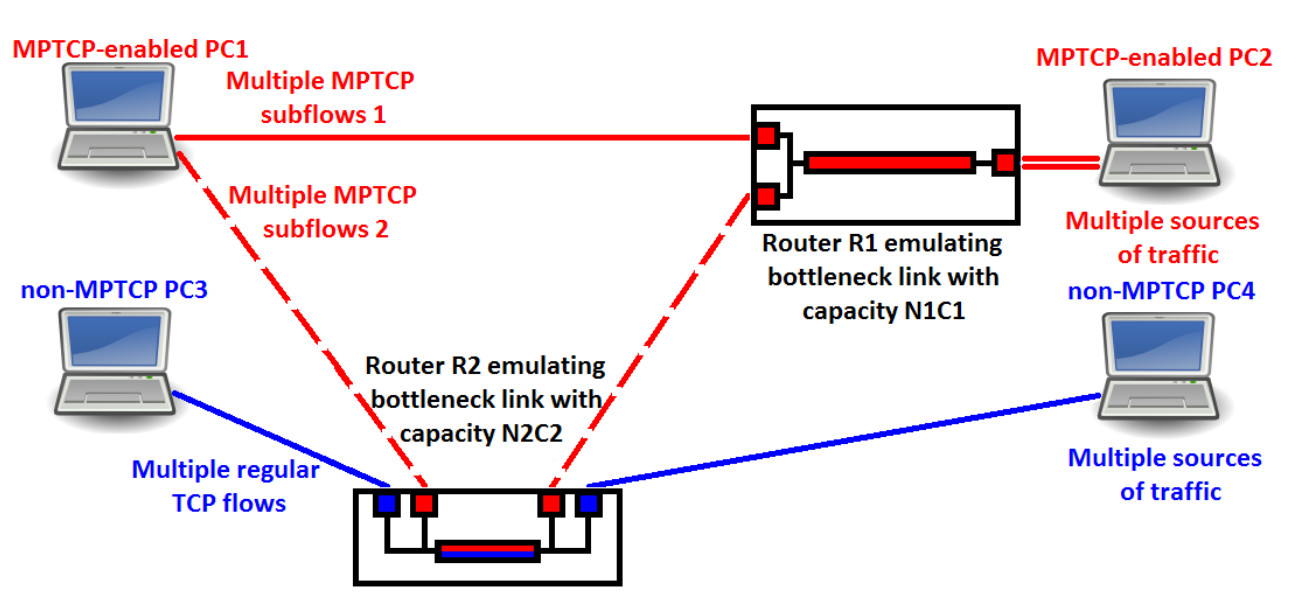
\includegraphics[width=0.6\textwidth]{../figures/khalili.jpg}
  \caption{\textbf{Testbed MPTCP vs TCP\cite{pareto2013}}.}
  \label{fig:khalili}
\end{figure}

Pour d�terminer les crit�res � respecter de l'ordonnanceur (celui par
d�faut, ou l'OLIA) et conserver les principes de MPTCP (�quitabilit�
avec les utilisateurs TCP et performances sup�rieures � TCP), nous
allons reproduire le \emph{testbed} utilis� dans l'article de Khalili
(\fig{fig:khalili}).


Si nous pouvons reproduire les r�sultats obtenus par Khalili avec
notre configuration, nous reproduirons le cas avec N1 utilisateurs
MPTCP et N2 utilisateurs TCP (voir \fig{fig:khalili2}).

\begin{figure}[!htb]
  \centering
  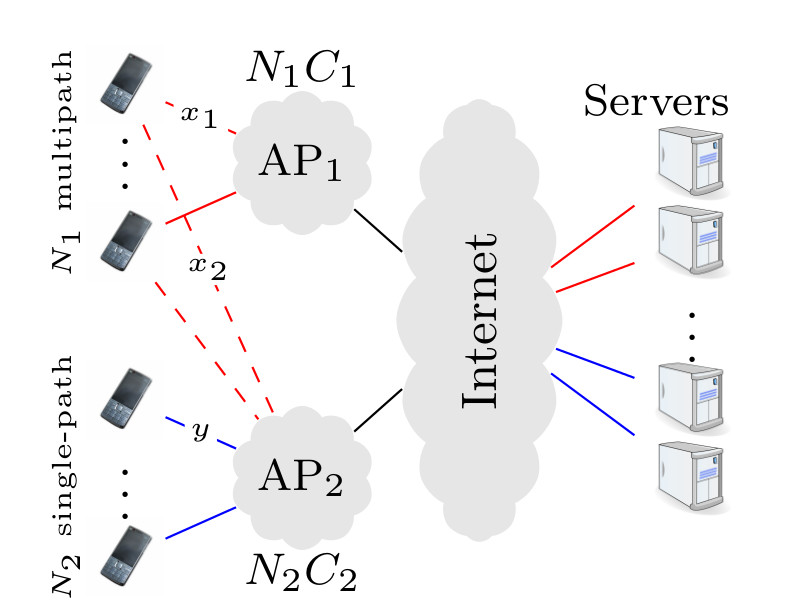
\includegraphics[width=0.4\textwidth]{../figures/khaliliB.jpg}
  \caption{\textbf{Testbed MPTCP vs TCP\cite{pareto2013}}. Les N1
    utilisateurs MPTCP (rouge) utilisent deux points d'acc�s pour se
    connecter � un serveur distant dont un qui est partag� avec les N2
    utilisateurs TCP (bleu).}
  \label{fig:khalili2}
\end{figure}

\subsection{Performances de MPTCP}
\label{sec:conce:perfMPTCP}

Pour mesurer les performances de MPTCP, nous allons faire varier les
propri�t�s de chaque sous-flot emprunt� en modifiant les chemins de
mani�re asym�trique. Le but est de cr�er des conditions de stress
qu'on pourra tester � la vol�e avec les diff�rents algorithmes g�rant
MPTCP (celui par d�faut, l'OLIA et le notre si celui-ci est
op�rationnel) et sur les diff�rentes topologies virtuelles construites.

Les contraintes appliqu�es auront comme crit�res la latence (crit�re
actuellement privil�gi� par l'ordonnanceur pour les choix de
sous-flots), la capacit�, le taux d'erreurs, la gigue, etc. Nous
testerons quelle est l'influence de ces param�tres sur le choix des
sous-flots par l'ordonnanceur.

\subsection{Conception algorithme s�curis�}
\label{sec:conc:algosec}

Le but est de rendre une connexion plus s�curis�e par la complexit� de
l'analyse des paquets de donn�es �chang�s entre deux
utilisateurs. Nous chercherons � faire une m�thode simple et non
performante pour effectuer des tests et savoir comment MPTCP r�agit au
nouvel algorithme de r�partition des paquets dans les sous-flots
TCP. Cette m�thode consiste � prendre le nombre de sous-flots total et
de r�partir les segments �quitablement entre les diff�rents
sous-flots. Le d�bit de chaque sous-flot correspondra au d�bit le plus
faible des sous-flots.  Cela reste une solution de l'objectif not�
dans le cahier des charges.

N�anmoins il sera n�cessaire d'avoir un algorithme plus
intelligent. En effet, il est n�cessaire d'avoir un meilleur
algorithme que celui expliqu� ci-dessus car la performance
pourrait �tre grandement affect�. Le d�bit pourrait �tre bien plus
faible qu'une connexion TCP classique sur le meilleur des chemins si
un des chemins a un d�bit beaucoup plus faible ou s'il est
congestionn�. Or m�me si nous voulons accro�tre la s�curit� il est
pr�f�rable d'avoir au moins le d�bit d'une connexion TCP simple. La
difficult� dans cette partie est de pouvoir adapter l'ordonnanceur
selon le nombre de sous-flots disponibles. Une id�e serait de r�partir
les charges de mani�re � que l'ordonnanceur de paquets n'envoie plus
de 50~+~$\varepsilon$~\% des segments � un unique sous-flot. Ce nombre
pourrait �tre variable selon d'autres param�tres comme le nombre de
sous-flots disponibles.


\subsection{Test de l'algorithme d'ordonnancement}
\label{sec:conc:ealgo}
L'�criture et le test de l'algorithme d'ordonnancement dans le noyau
linux peut s'av�rer une t�che difficile en si peu de temps. Pour
tester la validit� de notre algorithme d'ordonnancement, nous
r�fl�chissons � effectuer d'abord un \emph{proof of concept} en
utilisant directement python qui utilisera des fonctions de
\emph{callback} pour certaines fonctions du noyau n�cessaire �
MPTCP. On utilisera alors UDP pour la transmission des donn�es.

\clearpage

\section{\'Etat d'avancement}
\label{sec:etat-avancement}
\subsection[Outil de coordination: git]{Outil de coordination: git}
\label{subsec:etatavanc:git}
L'�tat des scripts utilis�es par l'�quipe est mise � jour par un
syst�me de version utilisant git
\url{https://github.com/Romain-Ly/PRES}.

\subsection[Compilation MPTC]{Compilation MPTCP\footnote{par M. Ly}}
\label{subsec:etatavanc:mininet-mptcp}

La mise en place du noyau linux MPTCP (v0.88) dans une VM de mininet
(v2.10) est � 100~\% termin�.

Les paquets debian pour l'installation du noyau MTPCP sur une VM de
mininet est disponible :
(\url{https://www.dropbox.com/sh/y4ykck8rg6908ps/7V3lsV6Ggg}).

Pour tester la r�ussite de l'installation, une topologie deux h�tes et
n switchs a �t� utilis�. L'utilisation de MPTCP montre un d�bit
sup�rieur lorsque l'on compare � la m�me exp�rience o� MPTCP a �t�
d�sactiv� dans le noyau.

\subsection[FatTree]{FatTree\footnote{par M. Ravier}}
\label{subsec:etatavanc:fattree}
Charg� de la conception du r�seau de test, ma premi�re pr�occupation a
�t� de ma�triser Mininet. Apr�s documentation, je me suis pench� sur
l'API Python offert par cet outil. Apr�s cette prise en main
concr�tis�e par quelques tests de connectivit� sur des topologies
simples, j'ai commenc� � coder ma propre topologie, un FatTree � 2
niveaux avec des switches � 36 ports. N'ayant pas trouv� de d�finition
formelle du FatTree, je me suis content� d'une instance particuli�re,
relativement simple mais permettant tout de m�me � MPTCP d'emprunter
plusieurs sous-flots diff�rents pour se rendre d'un h�te � l'autre.
Suite au travail de Romain, la prochaine t�che sera d'installer le
noyau MPTCP sur la machine virtuelle Mininet, de le configurer, puis
faire en sorte qu'il soit correctement utilis� dans notre r�seau
FatTree. J'effectuerai ensuite plusieurs tests de performance sur
cette topologie, probablement en collaboration avec Romain.

\subsection[Topologies virtualis�es]{Topologies
  virtualis�es\footnote{par M. Ly}}
\label{subsec:etatavanc:topologgie}

J'ai reproduit la topologie o� MPTCP est en concurrence avec un flux
TCP \cite{pareto2013}. Il reste � �tablir les tables de routage de
chaque h�te pour pouvoir tester les performances de MPTCP.


\subsection[Code MPTCP]{Code MPTCP\footnote{par M. Lam
    et M. Dubois}}
\label{subsec:etatavanc:mininet-mptcp}

Nous avons regard� les fichiers de MPTCP pour avoir une vision globale
de l'impl�mentation dans le noyau linux et essayer de d�terminer les
fichiers qui concernent l'ordonnancement des sous-flux.  Nous avons
ensuite essay� de d�terminer o� nous pouvions modifier le code afin
d'adapter l'ordonnanceur aux besoins du projet. Nous avons avanc� sur
cette phase de compr�hension du code mais il nous reste toujours �
savoir o� nous pouvons modifier le code sans rendre MPTCP non
fonctionnel ou non performant. Pour cela, il faudra tester sur des
topologies virtuelles simples et comparer les diff�rences de
performances. Bien s�r, dans les tests nous ne codons que des
ordonnanceurs idiots : ils effectueront uniquement une r�partition
�quitable des sous-flux sachant qu'ils ont tous le m�me d�bit.


\bibliography{./PRES}
\bibliographystyle{ieeetr}



\label{fin} %% Ne pas supprimer, n�cessaire pour calculer le nombre de pages RL
\end{document}


%%% Local Variables: 
%%% mode: latex
%%% TeX-master: t
%%% End: 
